% Created 2020-07-09 jue 18:01
% Intended LaTeX compiler: pdflatex
\documentclass[presentation,aspectratio=1610]{beamer}
\usepackage[utf8]{inputenc}
\usepackage[T1]{fontenc}
\usepackage{graphicx}
\usepackage{grffile}
\usepackage{longtable}
\usepackage{wrapfig}
\usepackage{rotating}
\usepackage[normalem]{ulem}
\usepackage{amsmath}
\usepackage{textcomp}
\usepackage{amssymb}
\usepackage{capt-of}
\usepackage{hyperref}
\usepackage{khpreamble}
\usepackage{amssymb}
\DeclareMathOperator{\shift}{q}
\DeclareMathOperator{\diff}{p}
\usetheme{default}
\author{Kjartan Halvorsen}
\date{2020-07-09}
\title{Control Computarizado - PID digital}
\hypersetup{
 pdfauthor={Kjartan Halvorsen},
 pdftitle={Control Computarizado - PID digital},
 pdfkeywords={},
 pdfsubject={},
 pdfcreator={Emacs 26.3 (Org mode 9.3.6)}, 
 pdflang={English}}
\begin{document}

\maketitle


\section{Discretization - repetición}
\label{sec:orge8b2768}
\begin{frame}[label={sec:orgf3e2bfa}]{Discretización de un controlador continuo}
\begin{center}
\includegraphics[width=0.7\linewidth]{../../figures/fig8-1.png}
\end{center}

\begin{itemize}
\item Dado un controlador obtenido de un diseño en tiempo continuo
\item Es necesario discretizarlo para implementar en una computadora
\end{itemize}
\end{frame}

\begin{frame}[label={sec:orgeaf9fa2}]{Métodos de discretización}
Introduciendo el operador diferencial:  \(\diff f(t) = \frac{d}{dt} f\)

\begin{enumerate}
\item Euler (diferencia hacia adelante) \(\diff \approx \frac{\shift -1}{h}\). Substituir
\[ s = \frac{z-1}{h} \] en \(F(s)\) para obtener
\[ F_d(z) = F(s')|_{s'=\frac{z-1}{h}}. \]
\item Euler hacia atras \(\diff \approx \frac{1 - \shift^{-1}}{h} = \frac{\shift -1}{h\shift}\). Substituir
\[ s = \frac{z-1}{zh} \] en \(F(s)\) para obtener
\[ F_d(z) = F(s')|_{s'=\frac{z-1}{zh}}. \]
\end{enumerate}
\end{frame}

\begin{frame}[label={sec:org485c545}]{Métodos de discretización}
\begin{enumerate}
\setcounter{enumi}{2}
\item El método de Tustin (transformada bilineal). Substituir
\[ s = \frac{2}{h}\frac{z-1}{z+1} \] en \(F(s)\) para obtener
\[ F_d(z) = F(s')|_{s'=\frac{2}{h}\cdot \frac{z-1}{z+1}}. \]
\item Discretización invariante a la rampa. Similar a discretización con ROC. La transformada z de una rampa es  \(\frac{zh}{(z-1)^2}\) y su transformada de Laplace \(1/s^2\). La discretización es dado por
\[ F_d(z) = \frac{(z-1)^2}{zh} \ztrf{\laplaceinv{\frac{F(s)}{s^2}}}. \]
\end{enumerate}
\end{frame}

\begin{frame}[label={sec:org651b3f6}]{Mapeo de la región estable del plano \(s\)}
\begin{center}
 \includegraphics[width=0.79\linewidth]{../../figures/fig8-2.png}\\
{\tiny Åström and Wittenmark \emph{Computer-controlled systems}}
\end{center}
\end{frame}

\begin{frame}[label={sec:org6b5f7e5}]{Forward difference exercise}
\begin{center}
\includegraphics[width=\linewidth]{../../figures/forward-diff-exercise}
\end{center}
\end{frame}
\begin{frame}[label={sec:org81ecf42}]{Backward difference exercise}
\begin{center}
\includegraphics[width=\linewidth]{../../figures/backward-diff-exercise}
\end{center}
\end{frame}


\section{PID}
\label{sec:orgb8042ca}
\begin{frame}[label={sec:orgd473c6a}]{PID tipo ISA}
ISA - International Society of Automation

\[ F(s) = K_c\left( 1 + \frac{1}{T_i s} + T_d s\right) \]

Con filtro pasobajo para la parte derivativo

\[ F(s) = K_c\left( 1 + \frac{1}{T_i s} + \frac{T_d s}{\frac{T_d}{N} s + 1}\right), \quad N \approx 3\; - \; 10 \]
\end{frame}

\begin{frame}[label={sec:org83b39d9}]{PID tipo ISA - parte derivativa}
\[ F(s) = K_c\left( 1 + \frac{1}{T_i s} + \frac{T_d s}{\frac{T_d}{N} s + 1}\right), \quad N \approx 3\; - \; 10 \]

\alert{Actividad en pares} Dibuja el diagrama de Bode (solo la magnitúd)  de la parte derivativa \[F_d(s) = \frac{T_d s}{\frac{T_d}{N} s + 1}\] usando las approximaciones de baja y alta frecuencia
\begin{align*}
 \text{$\omega$ small:} \quad & F_d(i\omega) \approx T_d i\omega \\
 \text{$\omega$ large:} \quad & F_d(i\omega) \approx \frac{T_d i \omega }{\frac{T_d}{N} i\omega} = N
\end{align*}
\end{frame}

\begin{frame}[label={sec:orgd46db42}]{PID tipo ISA - parte derivativa, solución}
\[ F(s) = K_c\left( 1 + \frac{1}{T_i s} + \frac{T_d s}{\frac{T_d}{N} s + 1}\right), \quad N \approx 3\; - \; 10 \]

\begin{center}
  \def\Td{1}
  \def\NN{6}
  \begin{tikzpicture}
    \begin{loglogaxis}[
    clip=false,
    width=14cm,
    height=5cm,
    ylabel={$|F_d(i\omega)|$},
    xlabel={$\omega$},
    ytick={\NN},
    yticklabels={$N$},
    xtick = {0.01, 0.1, 1, 10, 100}, 
    xticklabels={$\frac{0.01}{T_d}$, $\frac{0.1}{T_d}$, $\frac{1}{T_d}$, $\frac{10}{T_d}$, $\frac{100}{T_d}$},
    ]
      \addplot[red!80!black, no marks, domain=0.01:100, samples=20] {\Td*x/sqrt(1 + pow(\Td/\NN * x, 2))};
      \draw[orange, dashed] (axis cs: \NN/\Td, \NN) -- (axis cs: \NN/\Td, 0.003) node[below] {$\frac{N}{Td}$};
    \end{loglogaxis}

 \end{tikzpicture}
\end{center}
\end{frame}

\begin{frame}[label={sec:orgf2f216d}]{PID con accción derivada sobre la variable de proceso}
\begin{center}
  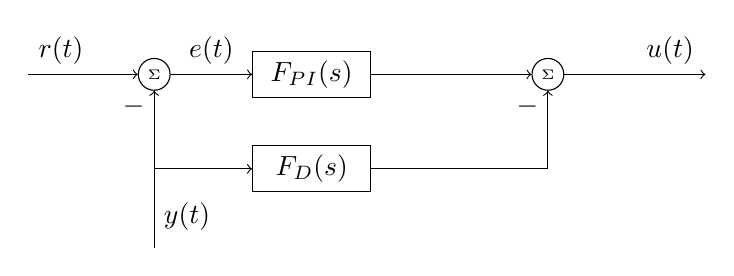
\begin{tikzpicture}[node distance=22mm, block/.style={rectangle, draw, minimum width=15mm}, sumnode/.style={circle, draw, inner sep=2pt}]

    \node[coordinate] (input) {};
    \node[sumnode, right of=input, node distance=16mm] (sum) {\tiny $\Sigma$};
    \node[block, right of=sum, node distance=20mm] (pi)  {$F_{PI}(s)$};
    \node[block, below of=pi, node distance=12mm] (dd)  {$F_{D}(s)$};
    \node[sumnode, right of=pi, node distance=30mm] (sum2) {\tiny $\Sigma$};
    \node[coordinate, below of=sum, node distance=22mm] (yy) {};
    \node[coordinate, right of=sum2, node distance=20mm] (output) {};

    \draw[->] (input) -- node[above, pos=0.3] {$r(t)$} (sum);
    \draw[->] (sum) -- node[above] {$e(t)$} (pi);
    \draw[->] (sum2) -- node[above, near end] {$u(t)$} (output);
    \draw[->] (yy) -- node[right, pos=0.2] {$y(t)$} node[pos=0.9, left] {$-$} (sum);
    \draw[->] (pi) -- node[above, near end] {} (sum2);
    \draw[->] (dd) -| node[left, pos=0.9] {$-$} (sum2);
    \draw[->] (yy) |- (dd);

  \end{tikzpicture}
\end{center}

\[ U(s) = \underbrace{K_c\left( 1 + \frac{1}{T_i s} \right)}_{F_{PI}(s)} E(s) - \underbrace{\frac{T_d s}{\frac{T_d}{N} s + 1}}_{F_{D}}Y(s)\]
\end{frame}

\section{Discretización del PID}
\label{sec:orgc5ba4c2}
\begin{frame}[label={sec:org7a89f5a}]{Discretización común del PID}
\begin{center}
  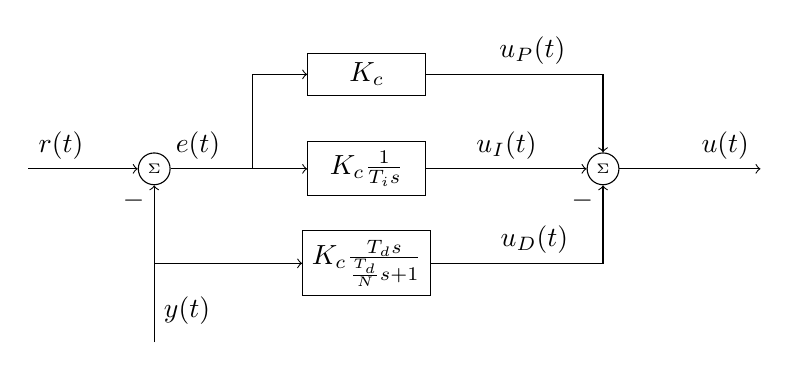
\begin{tikzpicture}[node distance=22mm, block/.style={rectangle, draw, minimum width=15mm}, sumnode/.style={circle, draw, inner sep=2pt}]

    \node[coordinate] (input) {};
    \node[sumnode, right of=input, node distance=16mm] (sum) {\tiny $\Sigma$};
    \node[block, right of=sum, node distance=27mm] (pi)  {$K_c\frac{1}{T_is}$};
    \node[block, below of=pi, node distance=12mm] (dd)  {$K_c\frac{T_d s}{\frac{T_d}{N} s + 1}$};
    \node[block, above of=pi, node distance=12mm] (pp)  {$K_c$};
    \node[sumnode, right of=pi, node distance=30mm] (sum2) {\tiny $\Sigma$};
    \node[coordinate, below of=sum, node distance=22mm] (yy) {};
    \node[coordinate, right of=sum2, node distance=20mm] (output) {};

    \draw[->] (input) -- node[above, pos=0.3] {$r(t)$} (sum);
    \draw[->] (sum) -- node[above, pos=0.2] {$e(t)$} node[coordinate, pos=0.6] (copy) {} (pi);
    \draw[->] (sum2) -- node[above, near end] {$u(t)$} (output);
    \draw[->] (yy) -- node[right, pos=0.2] {$y(t)$} node[pos=0.9, left] {$-$} (sum);
    \draw[->] (pi) -- node[above, ] {$u_I(t)$} (sum2);
    \draw[->] (dd) -| node[left, pos=0.9] {$-$} node[above, pos=0.3] {$u_D(t)$} (sum2);
    \draw[->] (yy) |- (dd);
    \draw[->] (pp) -| node[above, pos=0.3] {$u_P(t)$} (sum2);
    \draw[->] (copy) |- (pp);


  \end{tikzpicture}
\end{center}

\[ U(s) = U_P(s) + U_I(s) - U_D(s) = K_cE(s) + K_c\frac{1}{T_i s} E(s) - \frac{T_d s}{\frac{T_d}{N} s + 1}Y(s) \]

\alert{Actividad} 1) Usa \emph{Euler hacia adelante} para discretizar el parte integral y \emph{Euler hacia atrás} para discretizar el parte derivado. 2) Aplica la transformada z inversa para llegar a una ecuación de diferencias para el controlador.
\end{frame}

\begin{frame}[label={sec:org63a5a40}]{Discretización común del PID - Solución}
\begin{block}{La parte proporcional}
Facilísimo: \(u_P(kh) = K_c e(kh)\)
\end{block}
\begin{block}{La parte integral}
Substituye \(s = \frac{z-1}{h}\) en la funcion de transferencia \(F_I(s) = K_c \frac{1}{T_i s}\)
\[ F_{I,d}(z) = K_c\frac{1}{T_i \frac{z-1}{h}} = K_c \frac{\frac{h}{T_i}}{z-1}\]
\[U_I(z) = K_c \frac{\frac{h}{T_i}}{z-1} E(z), \qquad \text{}\]
\[U_I(z)(z-1) = K_c \frac{h}{T_i} E(z), \qquad \text{Aplica transformada z inversa}\]
\[ u_I(kh+h) - u_I(kh) = K_c \frac{h}{T_i} e(kh) \qquad \Leftrightarrow \qquad u_I(kh+h) = u_I(kh) + K_c\frac{h}{T_i} e(kh)\]
\end{block}
\end{frame}

\begin{frame}[label={sec:org931820e}]{Discretización común del PID - Solución}
\begin{block}{La parte derivativa}
Substituye \(s = \frac{z-1}{zh}\) en la funcion de transferencia \(F_D(s) = K_c \frac{T_d s}{\frac{T_d}{N} s + 1}\)
\[ F_{D,d}(z) = K_c\frac{T_d \frac{z-1}{zh}}{\frac{T_d}{N}\cdot\frac{z-1}{zh}+1} 
         = K_c \frac{T_d(z-1)}{\frac{T_d}{N}(z-1) + zh} 
= K_c \frac{T_d(z-1)}{(\frac{T_d}{N}+h)z -\frac{T_d}{N}} \]
\[ U_D(z) = K_c \frac{T_d(z-1)}{(\frac{T_d}{N}+h)z -\frac{T_d}{N}} Y(z)\]
\[ \Big((\frac{T_d}{N}+h)z -\frac{T_d}{N}\Big) U_D(z) = K_cT_d(z-1) Y(z), \qquad \text{aplica transformada z inversa} \]
\[ (\frac{T_d}{N}+h)u_D(kh+h) -\frac{T_d}{N}u_D(kh) = K_cT_d\big(y(kh+h) - y(kh)\big)\]
\end{block}
\end{frame}

\begin{frame}[label={sec:orgb9a4128}]{El algoritmo del PID discreto completo}
\begin{align*}
&\text{Dado:}  \;  y(kh-h), \; u_I(kh-h), \; u_D(kh-h)\\
& \text{\textcolor{green!60!black}{Toma de muestreos:}} \; r(kh), \; y(kh)\\
&e(kh) = r(kh) - y(kh)\\
&u_P(kh) = K_ce(kh)\\
&u_D(kh) = \frac{\frac{T_d}{N}}{\frac{T_d}{N} + h}u_D(kh-h) + K_c\frac{T_d}{\frac{T_d}{N} + h}\big(y(kh) - y(kh-h)\big)\\
&u(kh) = u_P(kh) + u_I(kh-h) + u_D(kh), \qquad \text{\textcolor{red}{Send to DAC}}\\
&u_I(kh) = u_I(kh-h) + K_c \frac{h}{T_i} e(kh)
\end{align*}

\begin{center}
  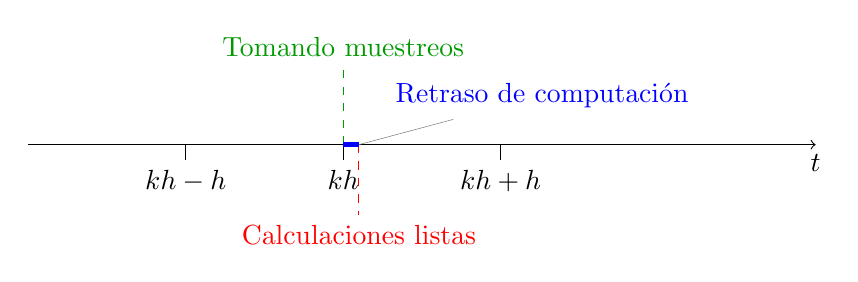
\begin{tikzpicture}
    \draw[->] (0,0) -- (10,0) node[below] {$t$};
    \draw (2,0) -- (2,-0.2) node[below] {$kh-h$};
    \draw (4,0) -- (4,-0.2) node[below] {$kh$};
    \draw (6,0) -- (6,-0.2) node[below] {$kh+h$};
    \draw[green!60!black, dashed] (4,0) -- (4, 1) node[above] {Tomando muestreos};
    \draw[red, dashed] (4.2,0) -- (4.2, -0.9) node[below] {Calculaciones listas};
    \draw[blue, ultra thick] (4,0) -- (4.2,0) node[coordinate, pin=45:{Retraso de computación}] {};
  \end{tikzpicture}
\end{center}
\end{frame}

\section{Sintonización de PID}
\label{sec:org09fad4a}
\begin{frame}[label={sec:org70fd43e}]{Sintonización de un PID}
\alert{El idéa} En forma experimental obtener unos pocos valores que capturan la dinámica del proceso. Usar una tabla predefinida para obtener las ganancias del PID dado estos valores.

Hay varios métodos. Ver el libro de texto y referencias incluidas.
\end{frame}

\begin{frame}[label={sec:org191fd9b}]{Sintonización de un PID - método de Smith \& Corripio}
Asuminedo modelo de proceso de primer orden con constante de tiempo \(T\) y retraso \(\tau\)
\[  \quad Y(s) = \frac{K_c\mathrm{e}^{-s\tau}}{sT + 1}U(s) \quad \overset{U(s) = \frac{u_f}{s}}{\Longrightarrow} \quad y(t) = u_f K_c\big( 1 - \mathrm{e}^{-\frac{t-\tau}{T}}\big)u_s(t-\tau)\]
\def\Tcnst{3}
\def\tdelay{0.6}
\def\ggain{2}
\def\uampl{0.8}
\pgfmathsetmacro{\yfinal}{\uampl*\ggain}
\pgfmathsetmacro{\yone}{0.283*\yfinal}
\pgfmathsetmacro{\ytwo}{0.632*\yfinal}
\pgfmathsetmacro{\tone}{\tdelay + \Tcnst/3}
\pgfmathsetmacro{\two}{\tdelay + \Tcnst}

\begin{center}
  \begin{tikzpicture}
    \begin{axis}[
    width=14cm,
    height=5cm,
    grid = both,
    xtick = {0, \tdelay, \tone, \two},
    xticklabels = {0, $\tau$, $\tau+\frac{T}{3}$, $\tau + T$},
    ytick = {0, \yone, \ytwo, \uampl, \yfinal},
    yticklabels = {0, $0.283y_{f}$, $0.632y_f$, $u_f$, $y_f$},
    xmin = -0.2,
    %minor y tick num=9,
    %minor x tick num=9,
    %every major grid/.style={red, opacity=0.5},
    xlabel = {$t$},
    ]
      \addplot [thick, green!50!black, no marks, domain=0:10, samples=100] {\uampl*\ggain*(x>\tdelay)*(1 - exp(-(x-\tdelay)/\Tcnst)} node [coordinate, pos=0.9, pin=-90:{$y(t)$}] {};
      \addplot [const plot, thick, blue!80!black, no marks, domain=-1:10, samples=100] coordinates {(-1,0) (0,0) (0,\uampl) (10,\uampl)} node [coordinate, pos=0.9, pin=-90:{$u(t)$}] {};
    \end{axis}
  \end{tikzpicture}
\end{center}

\[ y_f = \lim_{t\to\infty} y(t) = u_f K \quad \Rightarrow \quad K = \frac{y_f}{u_f}. \]
\end{frame}

\begin{frame}[label={sec:org883f4f7}]{Método de Smith \& Corripio - ejemplo}
\[  \quad Y(s) = \frac{K\mathrm{e}^{-s\tau}}{sT + 1}U(s) \quad \overset{U(s) = \frac{u_f}{s}}{\Longrightarrow} \quad y(t) = u_f K\big( 1 - \mathrm{e}^{-\frac{t-\tau}{T}}\big)u_s(t-\tau)\]
\def\Tcnst{2.1}
\def\tdelay{1}
\def\ggain{2}
\def\uampl{0.8}
\pgfmathsetmacro{\yfinal}{\uampl*\ggain}
\pgfmathsetmacro{\yone}{0.283*\yfinal}
\pgfmathsetmacro{\ytwo}{0.632*\yfinal}
\pgfmathsetmacro{\tone}{\tdelay + \Tcnst/3}
\pgfmathsetmacro{\two}{\tdelay + \Tcnst}

\begin{center}
  \begin{tikzpicture}
    \begin{axis}[
    width=12cm,
    height=4cm,
    grid = both,
    %xtick = {0, \tdelay, \tone, \two},
    %xticklabels = {0, $\tau$, $\tau+\frac{T}{3}$, $\tau + T$},
    %ytick = {0, \yone, \ytwo, \uampl, \yfinal},
    %yticklabels = {0, $0.283y_{f}$, $0.632y_f$, $u_f$, $y_f$},
    xmin = -0.2,
    minor y tick num=9,
    minor x tick num=9,
    every major grid/.style={red, opacity=0.5},
    %xlabel = {$t$},
    clip = false,
    ]
      \addplot [thick, green!50!black, smooth, no marks, domain=0:10, samples=16] {\uampl*\ggain*(x>\tdelay)*(1 - exp(-(x-\tdelay)/\Tcnst)} node [coordinate, pos=0.9, pin=-90:{$y(t)$}] {};
      \addplot [const plot, thick, blue!80!black, no marks, domain=-1:10, samples=100] coordinates {(-1,0) (0,0) (0,\uampl) (10,\uampl)} node [coordinate, pos=0.9, pin=-90:{$u(t)$}] {};
      \draw[thick, red, dashed] (axis cs: \tone, \yone) -- (axis cs: \tone, -0.45) node[below] {$t_1 = \tone = \tau + \frac{T}{3}$}; 
      \draw[thick, red, dashed] (axis cs: \tone, \yone) -- (axis cs: -1,\yone) node[left, anchor=east] {$0.283y_f = \yone$}; 
      \draw[thick, orange, dashed] (axis cs: \two, \ytwo) -- (axis cs: \two, -0.9) node[below] {$t_2 = \two = \tau + T$}; 
      \draw[thick, orange, dashed] (axis cs: \two, \ytwo) -- (axis cs: -1, \ytwo, -0.9) node[left, anchor=east] {$0.632y_f = \ytwo$}; 
      \draw[thick, green!70!black, dashed] (axis cs: 10, \yfinal) -- (axis cs: -1, \yfinal, -0.9) node[left, anchor=east] {$y_f = \yfinal$}; 
      \draw[blue!70!black, dashed] (axis cs: 0, \uampl) -- (axis cs: -1, \uampl, -0.9) node[left, anchor=east] {$u_f = \uampl$}; 
    \end{axis}
  \end{tikzpicture}
\end{center}
\[ \begin{cases} \tone = \tau + \frac{T}{3}\\ \two = \tau + T \end{cases} \quad \Rightarrow \quad \begin{cases} \tau = \tdelay \\ T = \Tcnst \end{cases}, \qquad  K = \frac{y_f}{u_f} = \frac{\yfinal}{\uampl} = \ggain \]
\end{frame}

\begin{frame}[label={sec:orgf203a01}]{Método de Smith \& Corripio - ejercicio}
\alert{Actividad} En grupos de dos: Comparte pantalla con esta diapositiva. Marca \(y_f\), \(0.632y_f\), \(0.283y_f\), \(u_f\), \(t_1\) y \(t_2\). Determina los parametros del modelo de primer orden con retraso.

\def\uampl{0.5}
\def\ttdelay{0.3}
\def\TTcnst{1.6}
\def\ggain{3}

\pgfmathsetmacro{\yfinal}{\uampl*\ggain}
\pgfmathsetmacro{\yone}{0.283*\yfinal}
\pgfmathsetmacro{\ytwo}{0.632*\yfinal}
\pgfmathsetmacro{\tone}{\tdelay + \Tcnst/3}
\pgfmathsetmacro{\two}{\tdelay + \Tcnst}


\begin{center}
  \begin{tikzpicture}
    \begin{axis}[
    width=13cm,
    height=6cm,
    grid = both,
    minor y tick num=9,
    minor x tick num=9,
    every major grid/.style={red, opacity=0.5},
    xlabel = {$t$},
    xmin = -1,
    ]
      \addplot [thick, green!50!black, no marks, domain=0:10, smooth, samples=16] {\uampl*\ggain*(x>\ttdelay)*(1 - (1+(x-\ttdelay)/\TTcnst)*exp(-(x-\ttdelay)/\TTcnst))} node [coordinate, pos=0.9, pin=-90:{$y(t)$}] {};
      \addplot [const plot, thick, blue!80!black, no marks, domain=-1:10, samples=100] coordinates {(-1,0) (0,0) (0,\uampl) (10,\uampl)} node [coordinate, pos=0.9, pin=-90:{$u(t)$}] {};
    \end{axis}
  \end{tikzpicture}
\end{center}
\end{frame}

\begin{frame}[label={sec:orgc81916a}]{Método de Smith \& Corripio - solución}
\end{frame}
\begin{frame}[label={sec:org71852b3}]{Método de Smith \& Corripio - Tabla de Ziegler-Nichols}
Dado el modelo 
\[ G(s) = K \frac{\mathrm{e}^{-s\tau}}{sT + 1} \]
Eliga sus parametros PID según la tabla de Ziegler-Nichols (1943)
   \begin{center}
   \setlength{\tabcolsep}{20pt}
   \renewcommand{\arraystretch}{1.5}
   \begin{tabular}{llll}
   Controlador & \(K_c\) & \(T_i\) & \(T_d\)\\
  \hline\hline
  P & \(\frac{T}{\tau K}\) &  & \\
  PI & \(\frac{0.9T}{\tau K}\) & \(\frac{\tau}{0.3}\) & \\
  PID & \(\frac{1.2T}{\tau K}\) & \(2\tau\) & \(\frac{\tau}{2}\)\\
  \hline
\end{tabular}
\end{center}

Funciona bien cuando \[0.1 < \frac{\tau}{T} < 0.6.\]
\end{frame}


\begin{frame}[label={sec:orga6d38fe}]{Tabla de  Ziegler-Nichols - ejemplo}
\[ G(s) = K \frac{\mathrm{e}^{-s\tau}}{sT + 1} = 2 \frac{\mathrm{e}^{-s}}{s2.1 + 1} \]
   \begin{center}
   \setlength{\tabcolsep}{20pt}
   \renewcommand{\arraystretch}{1.5}
   \begin{tabular}{llll}
   Controlador & \(K_c\) & \(T_i\) & \(T_d\)\\
  \hline\hline
  P & \(\frac{T}{\tau K} = \frac{2.1}{1 \cdot 2} = 1.05\) &  & \\
  PI & \(\frac{0.9T}{\tau K} = \frac{0.9\cdot 2.1}{2}= 0.945\) & \(\frac{\tau}{0.3} = \frac{1}{3} \) & \\
  PID & \(\frac{1.2T}{\tau K} = 1.26 \) & \(2\tau=2\) & \(\frac{\tau}{2}=\frac{1}{2}\)\\
  \hline
\end{tabular}
\end{center}
Regla de control (PID completo, \(N=10\)):
\[ U(s) = K_c\left( 1 + \frac{1}{T_i s} \right) E(s) - \frac{T_d s}{\frac{T_d}{N} s + 1}Y(s)
           =  1.26\left( 1 + \frac{1}{2 s} \right) E(s) - \frac{0.5s}{\frac{0.5}{10} s + 1}Y(s)\]
\end{frame}


\begin{frame}[label={sec:orgdaa3e58}]{Tabla de  Ziegler-Nichols - ejercicio}
Determina los parametros del PID para el modelo del ejercicio anterior \(\tau = 1.125\), \(T = 2.625\).

\[ G(s) = K \frac{\mathrm{e}^{-s\tau}}{sT + 1} =  \qquad\qquad\qquad\qquad\qquad\qquad \]
   \begin{center}
   \setlength{\tabcolsep}{20pt}
   \renewcommand{\arraystretch}{1.5}
   \begin{tabular}{llll}
   Controlador & \(K_c\) & \(T_i\) & \(T_d\)\\
  \hline\hline
  P & \(\frac{T}{\tau K} = \) &  & \\
  PI & \(\frac{0.9T}{\tau K} = \) & \(\frac{\tau}{0.3} = \) & \\
  PID & \(\frac{1.2T}{\tau K} = \) & \(2\tau\) & \(\frac{\tau}{2}=\)\\
  \hline
\end{tabular}
\end{center}
Regla de control (PID completo, \(N=?\)):
\[ U(s) = K_c\left( 1 + \frac{1}{T_i s} \right) E(s) - \frac{T_d s}{\frac{T_d}{N} s + 1}Y(s)
           =  \qquad\qquad\qquad\qquad\qquad\qquad\quad\quad\]
\end{frame}
\end{document}